\chapter{Einleitung}

Das Robot Operating System (ROS) ist eine Middleware um flexible Robotik Software zu schreiben. 2007 begann Willow Garage mit der Entwicklung von ROS und findet Heute in der Robotik Community weit verbreitet.
 Es liefert eine Sammlung von Tools, Libraries und Konventionen, welche das Erstellen von komplexer und robuster Robotik Software auf verschiedenen Platformen erleichtern soll.
ROS gliedert die Algorithmen zur Realisierung intelligenter Roboter in einzelne Aufgaben, welche durch jeweils einen Prozess (Node, Knoten) dargestellt und auf mehrere Rechner (Hosts) verteilt sein k�nnen.
Die Nodes verbinden sich nach dem Publisher-Subscriber Schema �ber ein Netzwerk miteinander um die Datenfl�sse herzustellen (ROS Graph).
Diese Grafen k�nnen allerdings sehr komplex werden.

\begin{figure}[H]
\centering
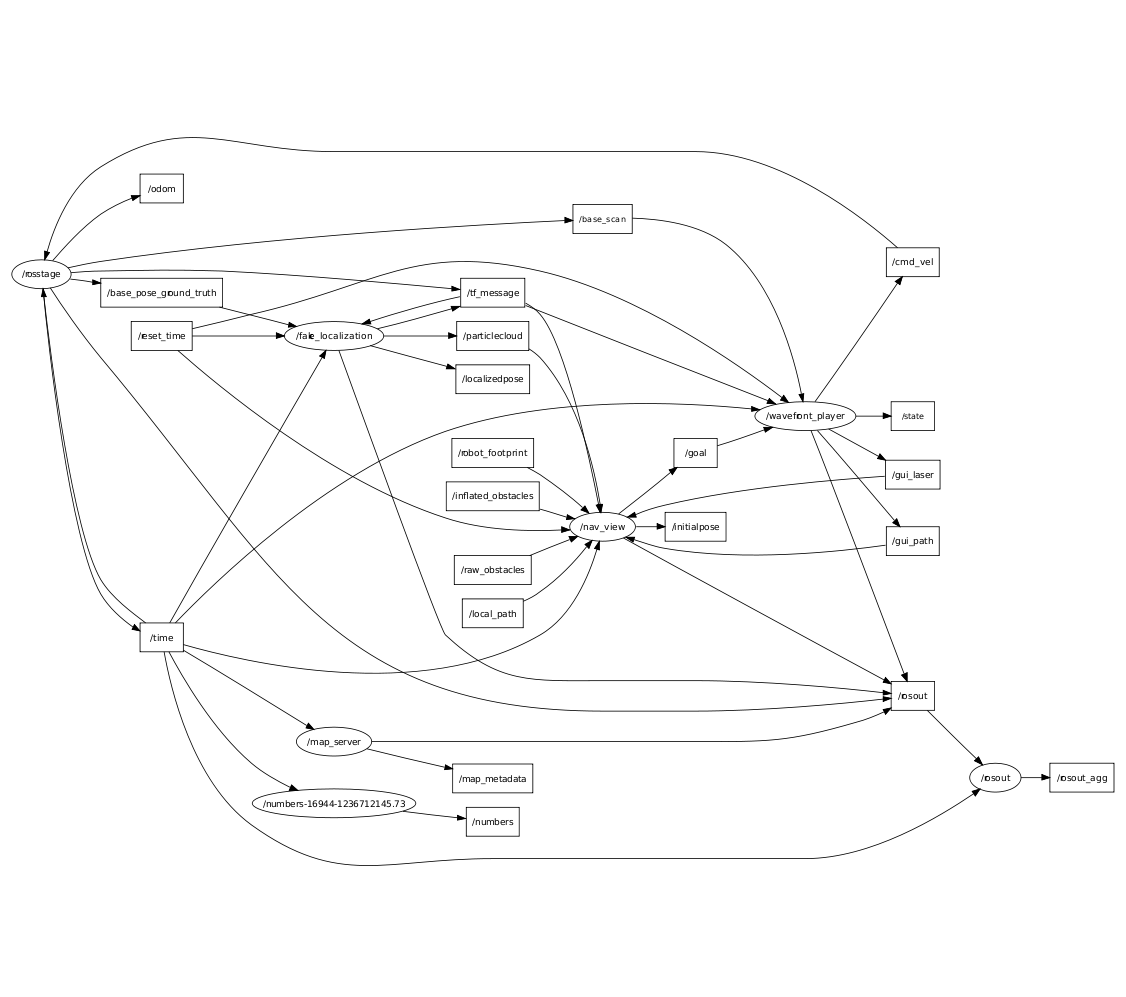
\includegraphics[scale=0.35]{./bilder/rxgraph.png} 
\caption{Beispiel eines ROS Graph. Nodes sind als Ellipsen, Topics als Rechtecke und Datenfluss als Pfeile dargestellt.
		Quelle: http://www.willowgarage.com }
\end{figure}

Ein Problem stellt die �berwachung dieses Systems dar. Zwar besteht im Moment die M�glichkeit, das Gesamtsystem auf Fehler zu �berpr�fen, jedoch ist es nicht m�glich zu bestimmen, 
welcher Knoten sich fehlerhaft verh�lt. Dies kann besonders bei gro�en System mit hunderten von Knoten zum Problem werden. Um ein schnelles Debuggen zu erm�glichen, bedarf es
einer Software zum dezentralen Erfassen der Fehlerursachen.


\vspace{0.5cm}

Unser Ziel als PSE-Team ist es, ein System zur Definiton des Soll-Zustandes und zum �berwachen des Ist-Zustandes individueller Knoten zu erstellen.
